%% \begin{figure}
%%   \begin{center}
%%     \begin{tabular}{c}
%%     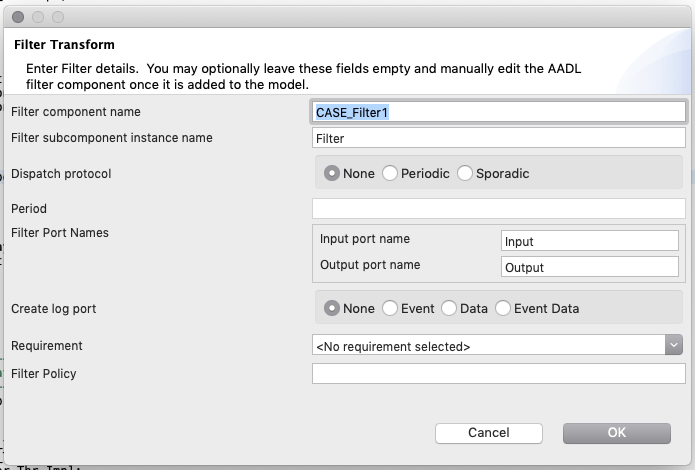
\includegraphics[scale=0.3]{dialogue.png}
%%     \end{tabular}
%%   \end{center}
%%   \caption{BriefCASE dialogue for filter transformation.}
%%   \label{fig:dialogue}
%% \end{figure}


Generally, AGREE contracts do not describe the computation that a
component performs. This is entirely by design: AGREE is intended to
be declarative and reasoning about component behavior takes place
solely at the specification level. It defines what a component
computes and not how it computes it. However, the syntax of AGREE
provides enough expressiveness to support the notion of a \emph{code
contract}: a contract from which an implementation can be
extracted. First we must discuss a class of guarantees---\emph{output
guarantees}---which determine the values on all output ports of a
component.

\begin{definition}[Output guarantee]
An \emph{output guarantee} is a stylized guarantee that fully
specifies the data written to an output port. There are three
possibilities according to whether the output port $p$ is
a \konst{data} port, an \konst{event} port, or an \konst{event data}
port:
\[
\begin{array}{ll}
\konst{data}: &  p = \mathit{e} \\
\konst{event}: &  \konst{event} (p) = \mathit{b} \\
\konst{event data}: & \itelse{b}{\konst{event} (p) \land p = e}{\neg \konst{event}(p)} \\
\end{array}
\]
\end{definition}

Informally, a code contract treats its \konst{eq} ``statements'' as
defining a list of assignments to state variables, and its output
guarantees as directives for producing output.

\begin{definition}[Code contract] A
  leaf component of the form $(I,O,A,P,\emptyset)$ is a
  \emph{code contract} if $\mathit{Eqs} \cup G \subseteq P$, where
\[\mathit{Eqs} = \set{v_1 = e_1, \cdots , v_n = e_n} \] is a non-empty set
of \konst{eq} statements and $G$ is the set of output guarantees, one for
each element of $O$. In the interpretation as code, the order of
elements of $\mathit{Eqs}$ is important, and is simply taken to be the
occurrence order of the \konst{eq} statements in the syntax. Thus we
will work with the
\emph{list} of equations $\mathit{Eqs} = [v_1 = e_1; \cdots ; v_n = e_n]$.
\end{definition}


The semantics of \secref{sec:agree-semantics} supports a formal
connection between the original contract---and verification results of
the AGREE model checker being run on it---and code generated from
specifications of leaf level cyber-components. It also provides the
root meaning at the base of a chain of translation steps moving from
an AGREE contract to a CakeML executable.

The first step in the chain maps the contract to a code-focused
representation. Assume given a code contract
$(I,O,A,\mathit{Eqs} \cup G \cup P,\emptyset)$, environment $E$, and
time $t$. The \emph{evaluation} of $\mathit{Eqs}$ followed by the
evaluation of $G$ results in a new environment $E'$ where the stream
values for state variables and outputs have been computed for time
$t$. The step from $E$ to $E'$ is one full cycle in the repeated
evaluation of the component.

\begin{definition}[Evaluation]
We overload existing notation and write the evaluation of
$\mathit{Eqs}$ and then $G$ in environment $E$ at time $t$ as
$\sem{\mathit{Eqs}\cdot G}^E_t$. The evaluation of $v = e \in {\Eqs}$
is an environment transformation
\[
 \sem{v = e}^E_t = E[v(t) \mapsto\sem{e}^E_t] \ .
\]
modifying $E$ so that stream $v$ has value $\sem{e}^E_t$ at time $t$.
The list {\Eqs} is evaluated by folding the transformation left-to-right
through it. The transformation is similarly applied to the list of output
guarantees $G$, computing the values on output ports. The details are
omitted, being a bit messy because of the different kinds of output
ports available.
\end{definition}


\begin{definition}[Code contract correctness]
Assume code contract $(I,O,A,\mathit{Eqs} \cup G \cup P,\emptyset)$.
The contract is \emph{correct}, if for all $E$ and $t$, whenever the
assumptions (historically) hold in $E$ and evaluation steps from $E$
to $E'$, then the guarantees hold in $E'$:
\[
\sem{\konst{Hist}(A)}^E_t \land E' = \sem{\mathit{Eqs} \cdot G}^E_t \imp \sem{P}^{E'}_t
\]
\end{definition}

How does this notion of correctness integrate with the verification
conditions generated by AGREE? In \emph{contract correctness}, the
model checker is proving the following property
\[
\konst{Hist}(A) \imp P
\]
and in \emph{code contract correctness} we essentially prove a Hoare
triple of the form
\[
\set{\konst{Hist}(A)}\; (\mathit{Eqs} \cdot G) \; \set{P}
\]
This accords with intuition, namely that AGREE is a kind of
`program-free program logic'; by pulling out a program
$(\mathit{Eqs}\cdot G)$ from a code contract we find ourselves in the
domain of imperative program verification. For example, at this
point one could apply a verification condition generator to help break
down the proof obligation. In order to use the code contract result in
system contract verification conditions, one has to show that the code
contract result implies the system verification condition.

\subsubsection*{Imperative code contracts.}

Stream-based evaluation allows values arbitrarily `deep in the past'
to be accessed by use of $\konst{pre}(-)$. However, the programming
languages targeted by SPLAT do not directly support streams.  We are
developing a translation to eliminate such deep temporal accesses by
the introduction of intermediate variables. The essential property the
translation needs to satisfy is a syntactic restriction ---call
it \emph{Pascalish}---that supports easy translation to standard
imperative languages.  The guiding intuition is that a Pascalish
{\Eqs} accesses at most one step in the past; also, accesses to a
past value of a variable are only possible until the variable is
updated. In informal terms, this means that ${\Eqs}\cdot G$ in a code
contract has the following properties:
\begin{itemize}
\item Followed-by only occurs at the top level of a variable definition, \eg, $v = e_1 \to e2$;
\item $\konst{pre}(e)$ is allowed only when $e$ is a variable; and
\item $\konst{pre}(v)$ is allowed only before the defining equation $v = e$ (and may occur in $e$).
\end{itemize}
For example, the Fibonacci sequence $1,1,2,3,5,8,13,\ldots$ can be
defined, albeit in a non-Pascalish manner, by
{\small
\begin{lstlisting}[style=agree]
  Fib = 1 -> pre(1 -> Fib + pre Fib)
\end{lstlisting}
}
\noindent or by (again non-Pascalish)
{\small
\begin{lstlisting}[style=agree]
  N = 0 -> 1 + pre(N)
  Fib = if N <= 1 then 1 else pre(Fib) + pre(pre(Fib))
\end{lstlisting}
}
\noindent or by (Pascalish):
{\small
\begin{lstlisting}[style=agree]
  N = 0 -> 1 + pre(N)
  F2 = 42 -> pre(F1)
  F1 = 42 -> pre(Fib)
  Fib = if N <= 1 then 1 else F1 + F2
\end{lstlisting}
}
(Note that the initial values of \verb+F1+ and \verb+F2+ are never
accessed, so 42 could be replaced by any number in their defining
equations.) A Pascalish ${\Eqs} \cdot G$ is straightforward to
implement in conventional programming languages, as we will see in
Section \ref{sec:synthesis}.

\subsection{Code contracts for the hardened system}
\label{sec:ha-contracts}

\newsavebox{\flt}
\begin{lrbox}{\flt}
  \begin{lstlisting}[style=agree,numbers=left] -- start user
    -- start user definitions
    eq policy : bool =
      WELL_FORMED_AUTOMATION_RESPONSE(Input);
    -- end user definitions

    guarantee "Filter output is well-formed" :
      if event(Input) and policy then
        event(Output) and Output = Input
      else
        not event(Output);
  \end{lstlisting}
\end{lrbox}

\newsavebox{\mntr}
\begin{lrbox}{\mntr}
  \begin{lstlisting}[style=agree,numbers=left]
    const is_latched : bool = true;

    -- start user definitions
    assume "One automation request in flight at a time" : *\label{line:mon-assume}*
      true -> (req => pre(Historically(not req) or Since(not req, rsp)));

    const MAX_LATENCY : int = 1; *\label{line:mon-const}*

    eq rsp : bool = event(Response);
    eq req : bool = event(Request);

    eq preIsPending : bool = false -> pre(isPending);*\label{line:mon-pre-pending}*
    eq isPending : bool = Since(not rsp, req and not rsp);*\label{line:mon-pending}*
    eq latency : int = 0 -> (if req then 0 else pre(latency) + 1);*\label{line:mon-latency}*

    eq policy : bool = (rsp => req) -> *\label{line:mon-policy}*
                         (    (isPending => latency < MAX_LATENCY)
                          and (rsp => (req or preIsPending)));
    -- end user definitions

    eq alert : bool = (not policy) -> *\label{line:mon-alert}*
                        ((is_latched and pre(alert)) or not policy);

    guarantee "Alert port tracks alert variable" :
      event(Alert) = alert;
    guarantee "Output if not alerted" :
      if (not(alert) and rsp) then
          event(Output) and (Output = Response)
      else
          not (event(Output));
  \end{lstlisting}
\end{lrbox}

\begin{figure}
  \begin{center}
    \begin{tabular}{c}
      \scalebox{0.62}{\usebox{\flt}} \\
    \end{tabular}
  \end{center}
  \caption{Code contract for high-assurance filter.}
  \label{fig:filter}
\end{figure}

\begin{figure}
  \begin{center}
    \begin{tabular}{c}
    \scalebox{0.62}{\usebox{\mntr}} \\
    \end{tabular}
  \end{center}
  \caption{Code contract for high-assurance monitor.}
  \label{fig:monitor}
\end{figure}

Code contracts for the filter and monitor are shown in
\figref{fig:filter} and \figref{fig:monitor}.
The filter is direct: it defines the policy according to the
well-formed requirement for data.  We now discuss the monitor in some
detail.

The monitor informally behaves as follows: if the \emph{policy} is
obeyed in the current step, and the alert has not yet been raised,
then the \texttt{Response} input is sent out on \texttt{Output}, and
the \texttt{Alert} output stays
low \lineref{line:mon-alert}. Otherwise \texttt{Alert} goes high and
stays high, and there is nothing sent henceforth on \texttt{Output}.

The \texttt{alert} variable (distinct from the \texttt{Alert} port)
depends not just on the policy but also on the
\texttt{is\_latched} constant, which has been set at configuration time.
Since \texttt{is\_latched} is \konst{true}, the alert is persistent,
meaning that once the alert is raised, it is always raised; otherwise,
it is the complement of the policy value in the current step.

The monitor policy is defined by marking, with variable \texttt{isPending},
when a request is made but not yet satisfied, and by counting the
number of steps (\texttt{latency}) between
requests. See \linesref{line:mon-pre-pending}{line:mon-latency}:
The \texttt{isPending} variable is true whenever there is a request
that does not coincide with a response, \ie, \texttt{isPending} holds
when \emph{there is no response since the most recent request without
a corresponding response}.  The
\texttt{latency} variable starts at zero, resets on every request, and
otherwise increments by one.  Note that the \texttt{preIsPending}
variable is a temporary needed to make the contract \emph{Pascalish};
otherwise, the current and previous value of \texttt{isPending} would
be simulataneously accessed in the definition of \texttt{policy}.

The policy (\lineref{line:mon-policy}) makes sure the latency is
bounded whenever there is a pending request, and it ensures that a
response is a result of a request.  The initial step differentiates
from later steps in only needing to be sure a response is a result of
a request, both happening in the initial step.

The latency bound for the monitor is defined by the constant
\texttt{MAX\_LATENCY} (\lineref{line:mon-const}).  In this example the
constant is set to one to be consistent with the system specification from the
previous section.  At time zero the policy is trivial: a response
requires an accompanying request.  After time zero, if a request is
pending in the current time step, then the latency must still be under
the bound, and if there is a response, then it closes a request now or
a pending request from earlier in time.

The policy definition only works if there is never more than one
outstanding request at a time; otherwise, the latency counter resets
incorrectly.  That requirement is encoded in the assumption
(\lineref{line:mon-assume}) and is the same assumption used for the
system input.  In fact, the policy can be written without the assumption, but
the policy is much simpler to write with the assumption.

As shown in \figref{fig:hardened-certificate}, the cyber-hardened
system passes AGREE verification.  That means that the high-assurance
components protect the WM from the untrusted AI generating malformed
data, spontaneous responses, or delayed responses.  Synthesis must
generate faithful implementations of the code contracts for the AGREE
verification result to apply to the deployed system.
